\begin{frame}[parent={ie:agenda}, hasnext=false, hasprev=false]
	\frametitle{Modelo de McCall}

	\begin{block:concept}{Modelo de McCall}
		\begin{itemize}
			\item Desenvolvido para a Força Aérea Norte-Americana
			\item Organizado em:
			\begin{itemize}
				\item Fatores: visão externa do software (usuários).
				\item Critérios: visão interna do software (desenvolvedores).
				\item Métricas
			\end{itemize}
		\end{itemize}
	\end{block:concept}
\end{frame}


\begin{frame}[hasnext=true, hasprev=true]
	\frametitle{Modelo de McCall}

	\begin{block:fact}{Pontos de vista}
		Fatores e critérios relacionados a três pontos de vista:
		\begin{itemize}
			\item Operação/uso do produto;
			\item Revisão/mudança do produto;
			\item Transição do produto.
		\end{itemize}
	\end{block:fact}
\end{frame}


\begin{frame}
	\frametitle{Modelo de McCall}
	\framesubtitle{Fatores: Operação}

	\begin{block:concept}{Modelo de McCall}
		\centering
		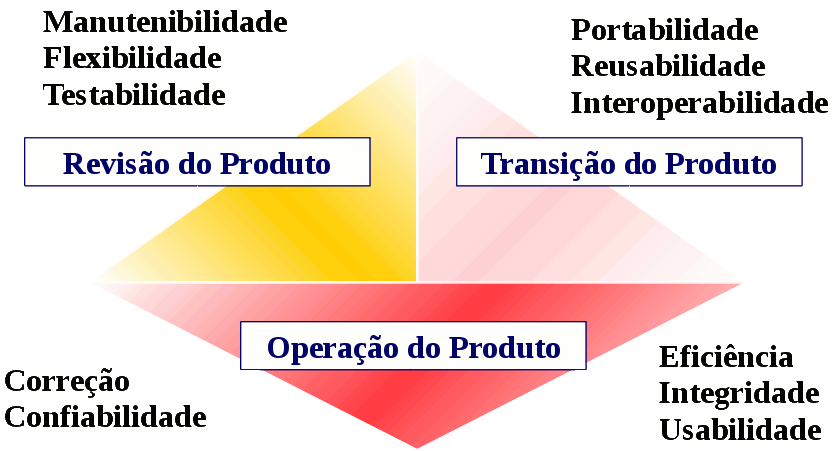
\includegraphics[width=.7\textwidth]{software-engineering/project-management/product/mccall/mccall}
	\end{block:concept}
\end{frame}


\begin{frame}
	\frametitle{Modelo de McCall}
	\framesubtitle{Fatores: Operação}
	
	\begin{block:concept}{Fatores de operação}
		\begin{itemize}
			\item \textbf{Correção}: Quanto um programa satisfaz sua especificação e cumpre os
			objetivos visados pelo cliente.
			\item \textbf{Confiabilidade}: Quanto que se pode esperar que um programa execute a
			função pretendida com a precisão exigida.
			\item \textbf{Eficiência}: Quantidade de recursos de computação e de código exigida
			para que um programa execute sua função.
			\item \textbf{Integridade}: Quanto o acesso ao software ou a dados, por pessoas
			não-autorizadas, pode ser controlado.
			\item \textbf{Usabilidade}: O esforço para aprender, operar, preparar a entrada e
			interpretar a saída de um programa.
		\end{itemize}
	\end{block:concept}
\end{frame}

\begin{frame}
	\frametitle{Modelo de McCall}
	\framesubtitle{Fatores: Revisão}

	\begin{block:concept}{Fatores de Revisão}
		\begin{itemize}
			\item \textbf{Manutenibilidade}: O esforço exigido para localizar e reparar erros
			em um programa.
			\item \textbf{Flexibilidade}: O esforço exigido para modificar um programa
			operacional.
			\item \textbf{Testabilidade}: O esforço exigido para testar um programa a fim de
			garantir que ele execute a função pretendida.
		\end{itemize}
	\end{block:concept}
\end{frame}


\begin{frame}
	\frametitle{Modelo de McCall}
	\framesubtitle{Fatores: Transição}

	\begin{block:concept}{Fatores de Transição}
		\begin{itemize}
			\item \textbf{Portabilidade}: O esforço exigido para transferir o programa de um
			ambiente de sistema de hardware e/ou software para outro.
			\item \textbf{Reusabilidade}: Quanto um programa (ou partes de um programa) pode 
			ser reutilizado em outras aplicações.
			\item \textbf{Interoperabilidade}: O esforço exigido para acoplar um sistema a
			outro.
		\end{itemize}
	\end{block:concept}
\end{frame}

\begin{frame}
	\frametitle{Modelo de McCall}
	\framesubtitle{Métricas}

	\begin{block:fact}{Atributos de qualidade medidos}
		\begin{columns}
			\column{.45\textwidth}
			\begin{itemize}
				\item Auditabilidade
				\item Acurácia
				\item Comunidade de Comunicação
				\item Inteireza
				\item Concisão
				\item Consistência
				\item Comunidade de Dados
				\item Tolerância a Erros
				\item Eficiência de Execução
				\item Expansabilidade
				\item Generalidade
			\end{itemize}
			
			\column{.45\textwidth}
			\begin{itemize}
				\item Independência de Hardware
				\item Instrumentação
				\item Modularidade
				\item Operabilidade
				\item Segurança
				\item Autodocumentação
				\item Simplicidade
				\item Independência de Software Básico
				\item Rastreabilidade
				\item Treinamento
			\end{itemize}
		\end{columns}
	\end{block:fact}
	
	\note{
		\begin{itemize}
			\item Auditabilidade - facilidade com que se pode checar a conformidade aos padrões.
			\item Acurácia - A precisão das computações e do controle.
			\item Comunidade de Comunicacão (Communication Commonality) - O grau em que as interfaces padrões, protocolos e larguras de banda (bandwidths) são usados.
			\item Inteireza - O quanto a implementação total da função requerida foi conseguida.
			\item Eficiência de Execução - O desempenho de run-time de um programa.
			\item Expansabilidade - O quanto o projeto arquitetural, procedimental e de dados podem ser ampliados.
			\item \ldots
			\item Generalidade - A amplitude de aplicação em potencial de componentes de programa.
			\item Modularidade - A independência funcional dos componentes do programa.
			\item Operabilidade - A facilidade de operação de um programa.
			\item Segurança - A disponibilidade de mecanismos que controlem ou protejam programas e dados.
			\item Autodocumentação - O quanto o código-fonte apresenta documentação significativa.
			\item Simplicidade - O quanto um programa pode ser entendido sem dificuldade.
			\item Independência do Software Básico - O quanto um programa é independente de particularidades não padronizadas de linguagens de programação non-standard, das características de sistemas operacionais e de outras sujeições ambientais.
			\item Rastreabilidade - A capacidade de rastrear uma representação de projeto ou componente de programa até os requisitos.
			\item Treinamento - O quanto o software auxilia no sentido de ajudar novos usuários a aplicarem o sistema.
			\item Independência de Hardware - O quanto o software é desvinculado do hardware em que opera.
			\item Instrumentação - O quanto o programa monitora sua própria operação e identifica erros que venham a ocorrer.
		\end{itemize}
	}
\end{frame}


\begin{frame}
	\frametitle{Modelo de McCall}
	\framesubtitle{Fatores e Métricas}

	\begin{block:fact}{``Métricas''}
		Define-se conjunto de medições para desenvolver expressões que poderão ser
		utilizadas para avaliar cada um dos fatores.
	\end{block:fact}
	
	\begin{block:fact}{}
		$F_q = \sum_{1}^m c_n \cdot m_n$, em que:
		\begin{itemize}
		 \item $F_q$ = fator de qualidade de software
		 \item $c_n$ = coeficiente de regressão
		 \item $m_n$ = métrica que afeta o fator de qualidade
		\end{itemize}
	\end{block:fact}
	
	\begin{block:fact}{}
		Total de fatores: 11
	
		Valores para $m_n$ são obtidos a partir de checklists, sendo graduados em
		0 a 10.
	\end{block:fact}
\end{frame}



\begin{frame}
	\frametitle{Modelo de McCall}
	\framesubtitle{Fatores e Métricas}

	\begin{block:fact}{}
		$F_q = \sum_{1}^m c_n \cdot m_n$
	\end{block:fact}

	\begin{block:fact}{}
		\centering
		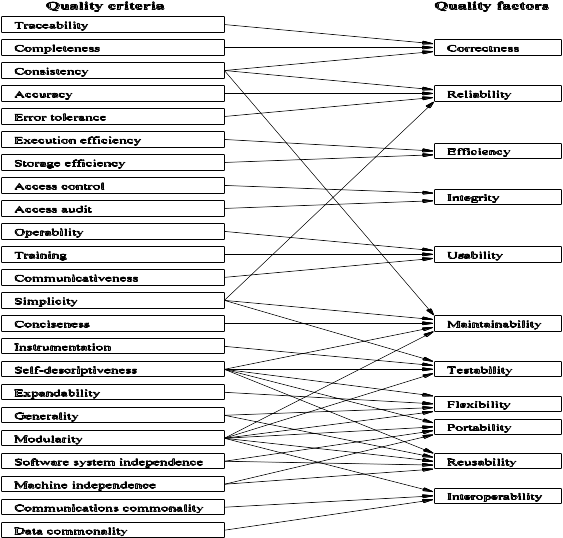
\includegraphics[width=.7\textwidth]{software-engineering/project-management/product/mccall/mccall-factor_metrics}
	\end{block:fact}
\end{frame}

